\section{Scalars}
\label{sec_scalars}

Example program which defines scalar field {\tt p}, assigns initial
values to it, and plots it, is given below ({\tt 06-01-main.cpp}):
%
{\small \begin{verbatim}
      1 #include "Include/psi-boil.h"
      2
      3 const real L =  6.2831853071796;
      4 const int  N = 64;
      5
      6 /****************************************************************************/
      7 main(int argc, char * argv[]) {
      8
      9   boil::timer.start();
     10
     11   /* plot in Tecplot format */
     12   boil::plot = new PlotTEC();
     13
     14   /* grid in "x", "y" and "z" direction */
     15   Grid1D g( Range<real>(0,L), N, Periodic::yes() );
     16
     17   /* computational domain */
     18   Domain d(g, g, g);
     19
     20   /* define unknowns */
     21   Scalar p(d); // pressure
     22
     23   /* assign initial values to pressure */
     24   for(int i=1; i<p.ni(); i++)
     25     for(int j=1; j<p.nj(); j++)
     26       for(int k=1; k<p.nk(); k++)
     27         p[i][j][k] = (1.0/16.0 )             *
     28                      (2.0 + cos(2.0*p.zc(k))) *
     29                      (cos(2.0*p.xc(i)) + cos(2.0*p.yc(j)));
     30
     31   /* plot scalar */
     32   boil::plot->plot(p, "pressure", 0);
     33
     34   boil::timer.stop();
     35   boil::timer.report();
     36 }
\end{verbatim}}
%
This program actually initializes {\tt p} according to:
%
\be
  p = \frac{1}{16} (2+cos(2 z)) (cos(2 x) + cos(2 y))
  \label{eq_pressure_init}
\ee

The program should be clear until line~21. Here is something new, field~{\tt p},
of type {\tt Scalar}, is defined from domain~{\tt d}. 

Since a {\tt Domain} in {\psiboil} is a {\em structured} entity, it has clearly 
defined extensions in $x$, $y$ and $z$ coordinate directions\footnote{Often denoted
as $i$, $j$ and $k$.}. {\tt Domain} has build in functions which give the resolution
in each direction, and these are: {\tt Domain::ni()}, {\tt Domain::nj()} and
{\tt Domain::nk()}. For this case, user specified resolution 64 in each coordinate
direction (lines~4 and~15). But, as it was explained in Sec.~\ref{sec_one-dimensional},
{\psiboil} adds two additional cells at the boundary of each coordinate direction,
meaning that {\tt Domain::ni()}, {\tt Domain::nj()} and {\tt Domain::nk()} hold the
value of~66. 

{\tt Scalar}, being defined for a {\tt Domain}, assumes the same structure as the
{\tt Domain}, and its values can be accessed with the usual {\tt C++} syntax
for three-dimensional arrays::
{\tt p[i][j][k];}
%
Furthermore, {\tt Scalar} has analogue member functions: {\tt Scalar::ni()}, 
{\tt Scalar::nj()} and {\tt Scalar::nk()} which define it's resolution\footnote{The
values obtained by {\tt Scalar}s {\tt ni()}, {\tt nj()} and {\tt nk()} are the
same as those obtained from the {\tt Domain} for which the scalar is defined.}.
Hence, to {\em browse} through all the values of {\tt Scalar p} over {\tt Domain d},
we use the triple loop in lines~24--26, using {\tt Scalar}'s member functions
{\tt ni()}, {\tt nj()} and {\tt nk()} to define ranges. 
%
This loop will browse from~1, which is the
first non-buffer cell in each direction, to~64, the last non-buffer cell in each
coordinate direction. By doing so, we browse exactly through 64 cells in each
direction, which is equal to the resolution specified by the user (line~4). 

This may quite look nice at the first glance, but is actually a {\em very dangerous}
practice. Imagine {\tt Domain} (which also reflects the {\tt Scalar}
changes internal structure in the future, and, instead of one, adds two layer of 
buffer cells at each end. 
All the loops in the program, having the form as the one given in lines~24--26 would fail! 
That should not come as a surprise, because the 1's that are used to specify the loop 
ranges in lines~24--26, are in essence, {\em ghost} numbers. 
To avoid this dangerous practice, {\tt Scalar} provides additional member functions: 
{\tt Scalar::si()} and {\tt Scalar::ei()} which mark the start and end of {\tt Scalar} 
cell range in $i$ direction (Analogue functions exist for $j$ and $k$ directions, of course.) 
Therefore, much safer variant of the loop, resilient to internal changes in
the objects {\tt Domain} and {\tt Scalar} would be:

\newpage

{\small \begin{verbatim}
     24   for(int i=p.si(); i<=p.ei(); i++) 
     25     for(int j=p.sj(); j<=p.ej(); j++) 
     26       for(int k=p.sk(); k<=p.ek(); k++) 
\end{verbatim}}

If the inner structure of {\tt Scalar} changes, it would reflected in its
{\tt si()}, {\tt ei()}, etc.\ and loops as this one would still work
properly. 

Since {\psiboil} is a three-dimensional program, triple loops like these occur very
frequently, which makes programming a tedious, lengthy and, let's face it, an 
error-prone task. Try to make a {\em small} error in line~25. Re-write it as:
%
{\small \begin{verbatim}
     25     for(int j=p.sj(); j<=p.ej(); i++) 
\end{verbatim}}
%
re-compile and re-run. You get a segmentation fault, only because you mistyped
{\tt j++} as {\tt i++}, an error which is easy to make, particularly if you have
plenty of triple loops all around the code. 

To avoid these sorts of errors, a special macro has been defined 
({\tt Scalar/scalar\_browsing.h}), which replaces the triple loop with
a single line (take the program {\tt 06-02-main.cpp}):
%
{\small \begin{verbatim}
     24   for_vijk(p,i,j,k)
\end{verbatim}}
%
which takes as parameters field over which you want to browse ({\tt p}), as 
well as counters in $i$, $j$ and $k$ direction ({\tt i}, {\tt j} and {\tt k}).
This macro reduces the size of the program and in that way reduces the chance
to make a typing error. 

One more detail remains to be explained at this point. To access cell-center
coordinates, {\tt Scalars}'s member functions: {\tt xc(int)}, {\tt yc(int)}
and {\tt zc(int)} should be used. In addition to these, there is a number
of other {\tt Scalars}'s member functions to access geometrical data, such 
as cell dimension ({\tt dxc()}, {\tt dyc()} and {\tt dzc()}), distance to neighboring
cell centers ({\tt dxe()}, {\tt dxw()} \ldots). All relevant information about
these functions is in the Doxygen documentation ({\tt PSI-Boil/Doc/Dox}). 

The pressure field prescribed by program ({\tt 06-02-main.cpp}) is shown in
Fig.~\ref{fig_pressure}.
%
%----------%
%          %
%  Domain  %
%          %
%----------%
\begin{figure}[ht]
  \centering
  \setlength{\unitlength}{1mm}
  \begin{picture}(100,85)(0,0)
    \thickbox{100}{85}
    \put(0,-3){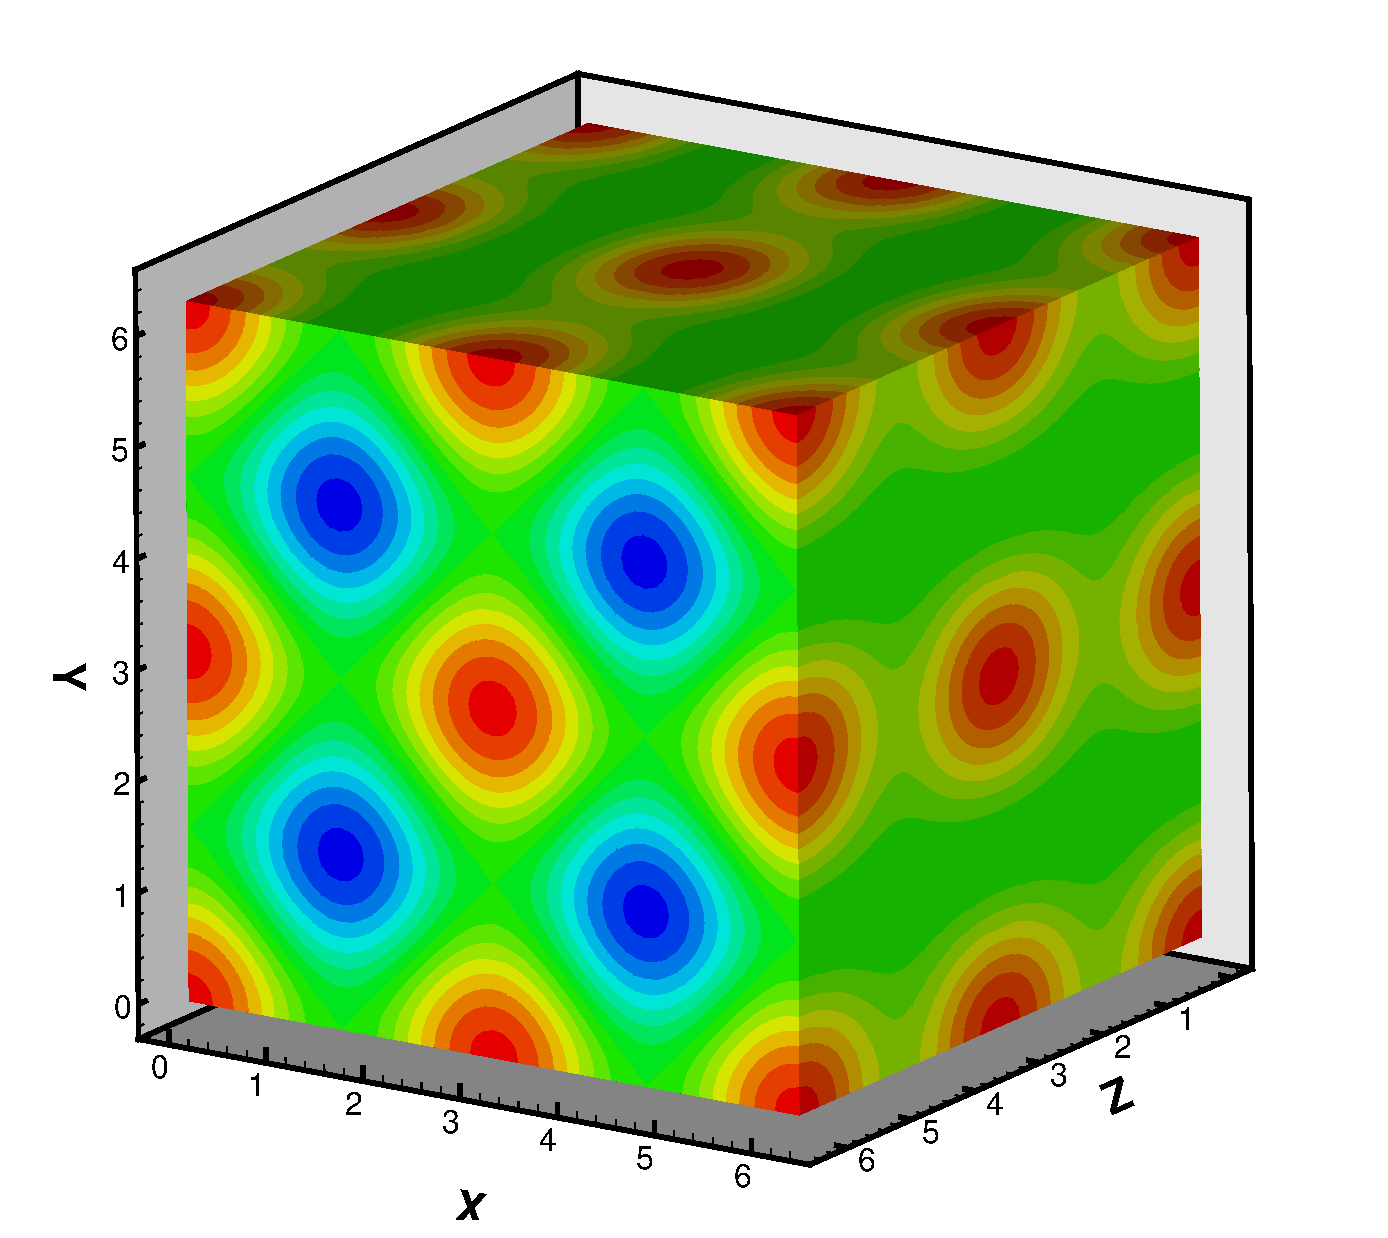
\includegraphics[scale=0.45]{Figures/06-01-pressure.eps}}
  \end{picture}
  \caption{Pressure field prescribed by Eq.~\ref{eq_pressure_init}}
  \label{fig_pressure}
\end{figure}

%---------------------------------------------------------------------nutshell-%
\vspace*{5mm} \fbox{ \begin{minipage}[c] {0.97\textwidth} %-----------nutshell-%
    {\sf Section \ref{sec_scalars} in a nutshell} \\  %---------------nutshell-%
   
      - Scalar fields are defined with {\psiboil} class {\tt Scalar}. \\

      - {\tt Scalar} is defined for a {\tt Domain}, with the constructor:
      \begin{itemize}
        \item {\tt Scalar(Domain \&);}
      \end{itemize}
 
      - {\tt Scalar}'s values are accessed with the usual {\tt C++} syntax:
      \begin{itemize}
        \item {\tt p[i][j][k];}
      \end{itemize}

      - To browse through all the {\tt Scalar} values, use the following macro:
      \begin{itemize}
        \item {\tt for\_vijk(Scalar \&, int i, int j, int k);}
      \end{itemize}
       Similar macros are defined in directory: {\tt PSI-Boil/Src/Field/Scalar/scalar\_browsing}. \\

      - {\tt Scalar} has a number of member functions to access {\tt Domain}s
      geometrical quantities. 
    
  \end{minipage} } %--------------------------------------------------nutshell-%
%---------------------------------------------------------------------nutshell-%
